% !TeX encoding = UTF-8
% !TeX program = xelatex
% !TeX spellcheck = fr_CA
\documentclass[nuit,charter,pied]{BeamerJS}
\title{Vecteurs aléatoires --- partie 2}
\subtitle{À l'intention des étudiants de STT-1500}
\institute{Université Laval}
\fonction{Département de mathématiques et de statistique}
\logotitre{../logo_UL.pdf}
\author{Jérôme Soucy}
\date{Hiver 2025}

\usepackage{adjustbox}
\usepackage{xstring}
\usepackage{commandesJS}
\addbibresource{../references.bib}
\NouvelleBoiteJS{rems}{Remarques}{Accent}{AccentBG}
\usepackage{calc}
\usepackage{nicefrac}
\usetikzlibrary{calc}
\usepackage{array}
\usepackage{booktabs}
\usepackage{relsize}
\usepackage{diffcoeff}
\usepackage{xfrac}
\begin{document}
\begin{frame}[plain,noframenumbering]
	\titlepage
\end{frame}

\begin{frame}{Résumé}
\tableofcontents
\end{frame}
\section{Espérance d'une fonction de variables aléatoires}
\begin{frame}{Théorème de changement de variable}
	\pause
	\begin{thm}
		Si $(X,Y)$ est un vecteur aléatoire, et si $g$ est une fonction réelle dont le domaine contient l'ensemble des valeurs possibles du couple $(X,Y)$, alors
		\[\Es{g(X,Y)}=\begin{cases}\sum_{(x,y)\in\R^2}g(x,y)p(x,y)&\text{dans le cas discret,}\\
			\int_{-\infty}^{\infty}\int_{-\infty}^{\infty}g(x,y)f(x,y)dxdy&\text{dans le cas abs. continu.}\\
		\end{cases}\]
		La fonction $p$ désigne la fonction de masse conjointe des variables aléatoires $X$ et $Y$ dans le cas discret, et la fonction $f$ désigne la fonction de densité conjointe des variables aléatoires $X$ et $Y$ dans le cas absolument continu.
	\end{thm}
\end{frame}
\begin{frame}{Conséquences sur l'espérance}
	\pause
	\begin{thm}
		Si $X_1,X_2,\ldots,X_n$ sont des variables aléatoires avec espérance finie, alors
		\[\Es{\sum_{k=1}^nX_k}=\sum_{k=1}^n\Es{X_k}.\]
		De plus, \textbf{si les variables $X_1,X_2,\ldots,X_n$ sont indépendantes}, alors
		\[\Es{\prod_{k=1}^nX_k}=\prod_{k=1}^n\Es{X_k}.\]
	\end{thm}
\end{frame}
\begin{frame}{Conséquences sur l'espérance --- suite}
	\pause
	\begin{thm}
		Si $X$ et $Y$ sont des variables aléatoires indépendantes, et si les espérances $\Es{h(X)}$ et $\Es{g(Y)}$ sont finies, alors
		\[\Es{h(X)g(Y)}=\Es{h(X)}\Es{g(Y)}.\]
	\end{thm}
\end{frame}
\section[f.g.m.]{Somme de v.a. et f.g.m.}
\begin{frame}{Somme de v.a. et f.g.m.}
	\pause
	Nous avons déjà vu que la fonction génératrice des moments d'une v.a. $X$ est définie par
	\[M_X(t)=\Es{e^{tX}}=\begin{cases}\sum_{x\in\R}e^{tx}p(x)&\text{dans le cas discret,}\\
		\int_{-\infty}^{\infty}e^{tx}f(x)dx&\text{dans le cas abs. continu.}
	\end{cases}\]
	Si on connait la f.g.m. d'une somme de variables aléatoires indépendantes, on peut parfois connaître la distribution de cette somme si on peut identifier la loi de distribution qui possède la f.g.m. trouvée. La f.g.m. de cette somme peut être calculée facilement si on connaît les f.g.m. des deux variables dont on veut en étudier la somme.
\end{frame}
\begin{frame}{Résultat}
	\begin{prop}
		Si $X_1,X_2,\ldots,X_n$ sont des variables aléatoires indépendantes avec respectivement $M_{X_1},M_{X_2},\ldots,M_{X_n}$ comme fonction génératrice des moments, alors la fonction génératrice des moments de la variable aléatoire \[S=\sum_{k=1}^nX_k\] est donnée par
		\[M_S(t)=\prod_{k=1}^n M_{X_k}(t).\]
	\end{prop}
\end{frame}

\begin{frame}[t]{La loi de Poisson}
	Supposons que $X_1, X_2,\ldots, X_n$ sont des v.a. i.i.d. (indépendantes identiquement distribuées) suivant une loi de Poisson de paramètre $\nu$. Trouvez la loi de la somme des $X_i$.
\end{frame}
\begin{frame}[t]{La loi exponentielle}
	Supposons que $X_1, X_2,\ldots, X_n$ sont des v.a. indépendantes dont la loi est l'exponentielle de paramètre $\lambda$. Trouvez la fonction génératrice de la v.a. $S=\sum_{k=1}^nX_k$.
\end{frame}

\section{Covariance et corrélation}
\begin{frame}{Définition}
	\pause
	\begin{defn}{}
		Soit $X$ et $Y$ des variables aléatoires. La covariance de $X$ et $Y$, notée $\Cov{X,Y}$, est définie par
		\[\Cov{X,Y}=\Es{(X-\mu_X)(Y-\mu_Y)}.\]
	\end{defn}
\end{frame}
\begin{frame}{Résultats}
	\pause
	\begin{prop}
		Soit $X$ et $Y$ des v.a., $a,b,c$ et $d$ des nombres réels. Alors
		\[\Cov{aX+b,cY+d}=ac\Cov{X,Y}.\]
	\end{prop}
	\begin{prop}
		Soit $X$ et $Y$ des v.a.. Un calcul direct montre que
		\[\Cov{X,Y}=\Es{XY}-\Es{X}\Es{Y}.\]
	\end{prop}
\end{frame}
\begin{frame}{Résultats --- cas des variables indépendantes}
	\pause
	\begin{prop}
		Soit $X$ et $Y$ des variables aléatoires indépendantes. Alors
		\[\Cov{X,Y}=0.\]
	\end{prop}
\begin{lumiere}
	$\Var{X}=\Cov{X,X}$
\end{lumiere}
\end{frame}


\begin{frame}{Covariance et variance}
	\begin{prop}
		Soit $X$ et $Y$ des variables aléatoires. Alors
		\[\Var{X+Y}=\Var{X}+2\Cov{X,Y}+\Var{Y}.\]
		Plus généralement, si $X_1,X_2,\ldots,X_n$ sont des variables aléatoires avec variance finie, alors
		\[\Var{\sum_{k=1}^nX_k}=\sum_{k=1}^n\Var{X_k}+2\sum_{1\leq i<j\leq n}^n\Cov{X_i,X_j}.\]
		Ainsi, si les $X_1,X_2,\ldots,X_n$ sont des variables aléatoires \textbf{indépendantes}, on peut conclure que la variance d'une somme est la somme des variances.
	\end{prop}

\end{frame}
\begin{frame}{Coefficient de corrélation}
	\pause
	\begin{defn}{}
		Soit $X$ et $Y$ des variables aléatoires telles que leur variance est strictement positive. On définit le coefficient de corrélation de $X$ et $Y$, noté $\rho_{X,Y}$, par
		\[\rho_{X,Y}=\frac{\Cov{X,Y}}{\sigma_X\sigma_Y}.\]
	\end{defn}
	Le coefficient de corrélation, tout comme la covariance, est une mesure du degré d'association linéaire de deux variables. L'avantage du coefficient de corrélation par rapport à la covariance est qu'il est normalisé: Il se situe toujours entre -1 et 1, et il n'a pas d'unité.
\end{frame}
\begin{frame}[t]{Un exemple}
	Supposons que $X$ soit une variable aléatoire uniforme sur l'intervalle $\intoo{0}{1}$. On défini $Y$ comme étant la variable aléatoire $1-X$. Calculez le coefficient de corrélation de $X$ et $Y$.\\
	\textbf{Solution}\\
	On déduit que $Y$ est aussi une uniforme sur l'intervalle $\intoo{0}{1}$ car elles ont la même densité.
	\begin{lumiere}
		L'espérance et la variance d'une v.a. uniforme sur $(a,b)$ sont respectivement $\frac{a+b}{2}$ et $\frac{(b-a)^2}{12}$.
	\end{lumiere}
D'une part,  on trouve que $\Es{X}=\Es{Y}=\sfrac{1}{2}$ et $\Var{X}=\Var{Y}=\sfrac{1}{12}$.
\end{frame}
\begin{frame}[t]{(suite)}
\begin{columns}[T,onlytextwidth]
\begin{column}{0.48\linewidth}
D'autre part, on trouve que
\begin{align*}
	\Cov{X,Y}&=\Es{XY}-\Es{X}\Es{Y}\\
	&=\Es{X(1-X)}-\sfrac{1}{2}\cdot\sfrac{1}{2}\\
	&=\Es{X}-\Es{X^2}-\sfrac{1}{4}\\
	&=-\sfrac{1}{12}.
\end{align*}
\end{column}
\begin{column}{0.48\linewidth}
	Ainsi,
	\begin{align*}
		\rho_{X,Y}&=\frac{\Cov{X,Y}}{\sigma_X\sigma_Y}\\[0.5cm]
		&=\frac{-\sfrac{1}{12}}{\sqrt{\sfrac{1}{12}}\cdot\sqrt{\sfrac{1}{12}}}\\[0.5cm]
		&=-1.
	\end{align*}
\end{column}
\end{columns}
\end{frame}
\begin{frame}{Coefficient de corrélation --- suite}
	\pause
	\begin{thm}
		Soit $X$ et $Y$ des variables aléatoires telles que $0<\sigma_X<\infty$ et $0<\sigma_Y<\infty$. Alors
		\begin{enumerate}
			\item $-1\leq \rho_{X,Y}\leq 1$\,;\
			\item $\rho_{X,Y}=1$ si et seulement si il existe des constantes $a$ et $b$, avec $a>0$, telles que $\P{Y=aX+b}=1$\,;\
			\item $\rho_{X,Y}=-1$ si et seulement si il existe des constantes $a$ et $b$, avec $a<0$, telles que $\P{Y=aX+b}=1$\,;\
			\item Si $a, b, c$ et $d$ sont des constantes, et si $a\neq 0$ et $c\neq 0$ sont de même signe, alors $\rho_{aX+b,cY+d}=\rho_{X,Y}$\,;\
			\item Si $a, b, c$ et $d$ sont des constantes, et si $a\neq 0$ et $c\neq 0$ sont de signe opposés, alors $\rho_{aX+b,cY+d}=-\rho_{X,Y}$\,;\
		\end{enumerate}
	\end{thm}
\end{frame}
\begin{frame}
	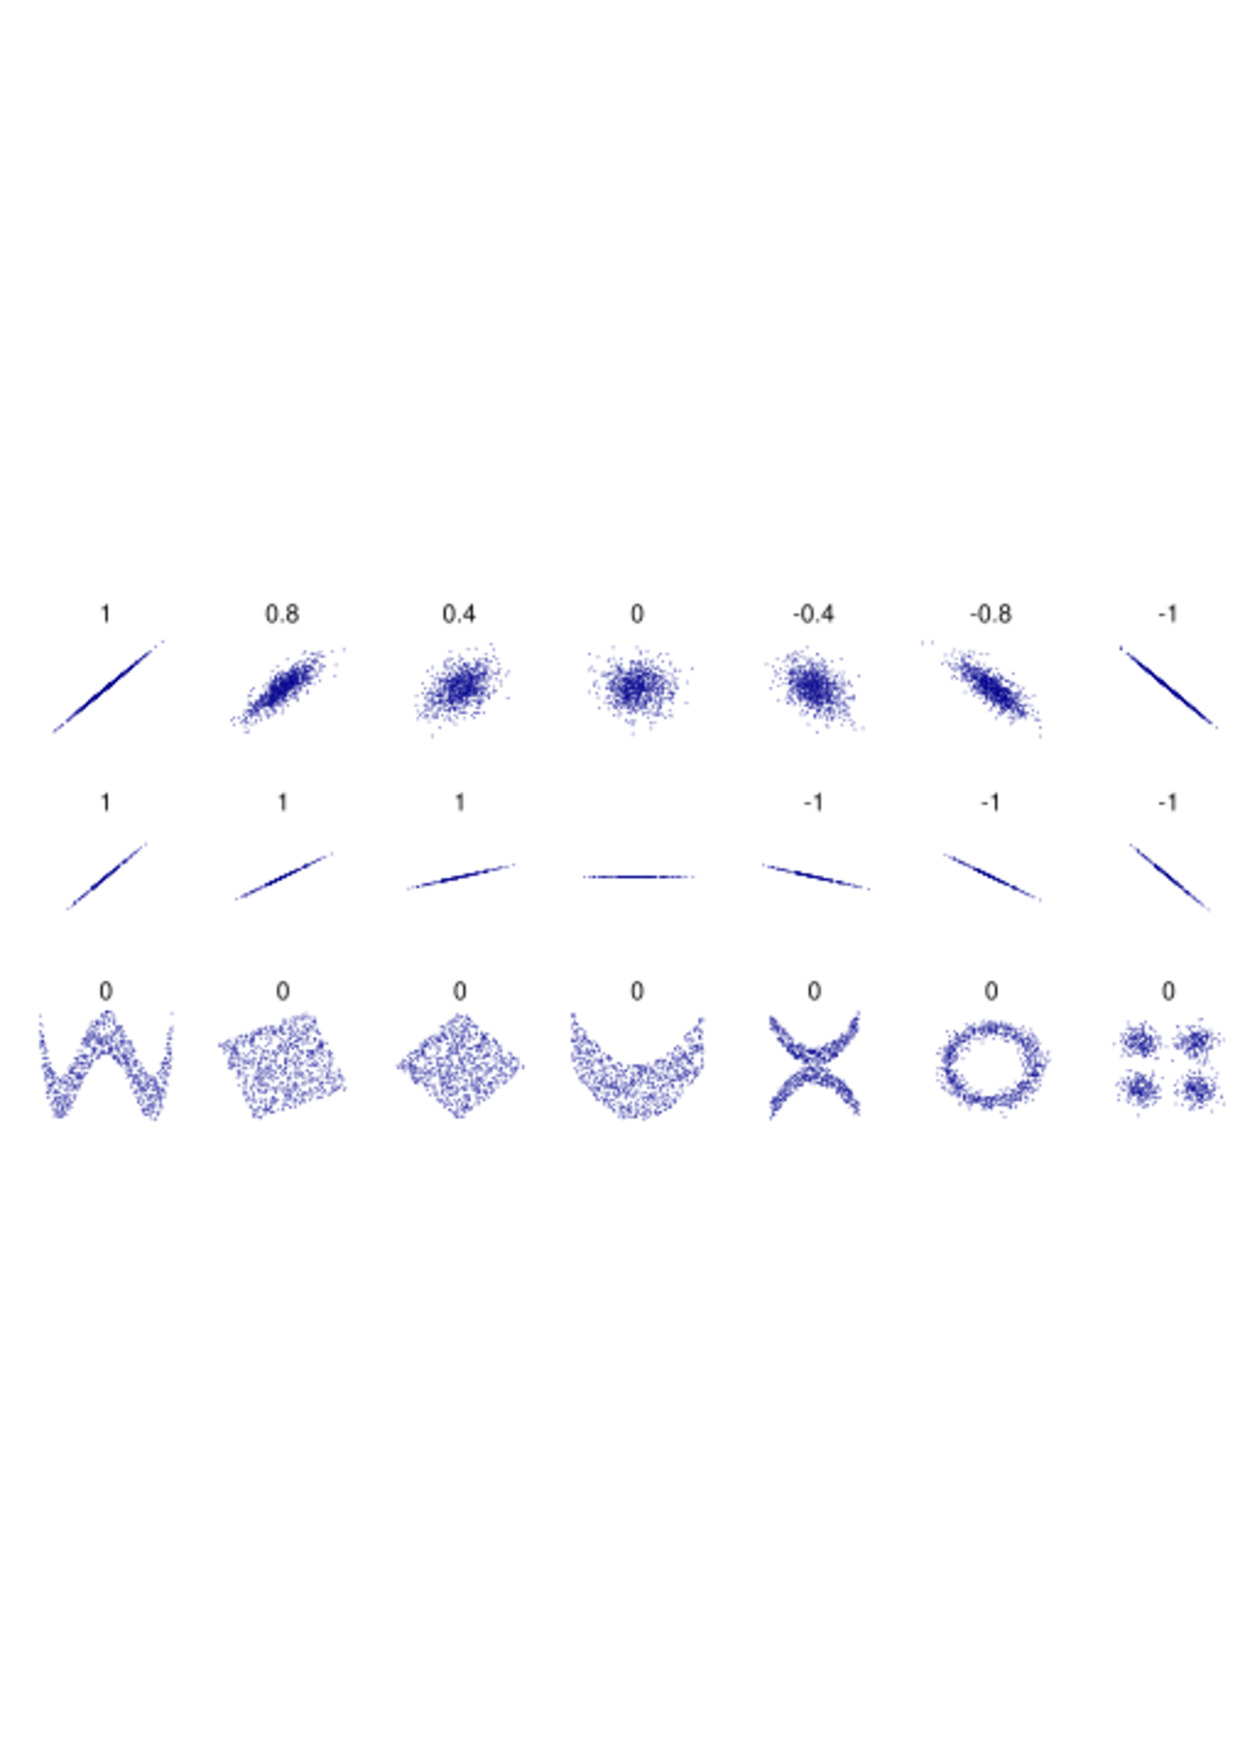
\includegraphics[width=\textwidth]{images/Correlation.pdf}
	\vfill
	\url{https://commons.wikimedia.org/w/index.php?title=File:Correlation_examples2.svg&oldid=696631151}
\end{frame}
\begin{frame}{Un exemple}
	On lance une pièce de monnaie $3$ fois. On note $X$ le nombre de fois où pile a été obtenu et on note $Y$ la longueur de la plus longue sous-suite composée uniquement du résultat pile. Par exemple, pour la suite $PPF$ on a que $X=2$ et $Y=2$ alors que pour $PFP$ on a que $X=2$ et $Y=1$. Calculez le coefficient de corrélation de $X$ et $Y$.
	
	Nous avons que 
	\[\rho_{X,Y}=\frac{\Cov{X,Y}}{\sigma_X\sigma_Y}.\]
	
	Calculons chacun des termes apparaissant dans cette expression.
\end{frame}
\begin{frame}[t]{Calcul de $\sigma_X$}
On constate que $X\sim \text{binomiale}\,\left(3,\frac{1}{2}\right)$.
\begin{lumiere}
	Rappel : la variance d'une v.a. de loi $\loibinomiale{n}{p}$ est $np(1-p)$.
\end{lumiere}
Ainsi,
\[\sigma_X=\sqrt{3\cdot\frac{1}{2}\cdot\frac{1}{2}}=\frac{\sqrt{3}}{2}.\]
\end{frame}
\begin{frame}[t]{Calcul de $\sigma_Y$}
	\small
	\begin{lumiere}
		Rappel : la variance d'une variable aléatoire $Y$ est
		$\Es{Y^2}-\Es{Y}^2$.
	\end{lumiere}

\begin{center}
\begin{tabular}{@{}cc@{}}
	\toprule
	Valeurs de $k$ & $\P{Y=k}$ \\ \midrule
	$0$            & $\sfrac{1}{8}$              \\
	$1$            & $\sfrac{4}{8}$              \\
	$2$            & $\sfrac{2}{8}$              \\
	$3$            & $\sfrac{1}{8}$              \\ \bottomrule
\end{tabular}\hspace{2cm}
\begin{tabular}{@{}cc@{}}
	\toprule
	Valeurs de $k$ & $\P{Y^2=k}$     \\ \midrule
	$0$            & $\sfrac{1}{8}$ \\
	$1$            & $\sfrac{4}{8}$ \\
	$4$            & $\sfrac{2}{8}$ \\
	$9$            & $\sfrac{1}{8}$	\\ \bottomrule
\end{tabular}
\end{center}
\[\Es{Y^2}-\Es{Y}^2=1\cdot\sfrac{4}{8}+4\cdot\sfrac{2}{8}+9\cdot\sfrac{1}{8}-\Bigl(\underbrace{1\cdot\sfrac{4}{8}+2\cdot\sfrac{2}{8}+3\cdot\sfrac{1}{8}}_{\Es{Y}=\sfrac{11}{8}}\Bigr)^2=\frac{47}{64},\]
d'où $\sigma_{Y}=\sqrt{47}/8$.

\end{frame}
\begin{frame}[t]{Calcul de $\Cov{X,Y}$}
	\small
	\begin{columns}[T,onlytextwidth]
	\begin{column}{0.58\linewidth}
	\begin{lumiere}
		$\Cov{X,Y}=\Es{XY}-\Es{X}\Es{Y}$
	\end{lumiere}
	Les valeurs possibles pour $X$ et $Y$ sont $0,1,2$ et $3$. Les valeurs possibles pour $XY$ sont $0,1,4$ et $9$ ($6$ n'est pas une valeur possible).
	\end{column}
	\begin{column}{0.38\linewidth}
	\centering
	\begin{tabular}{@{}cc@{}}
		\toprule
		Valeurs de $k$ & $\P{XY=k}$     \\ \midrule
		$0$            & $\sfrac{1}{8}$ \\
		$1$            & $\sfrac{3}{8}$ \\
		$2$            & $\sfrac{1}{8}$ \\
		$4$            & $\sfrac{2}{8}$ \\ 
		$9$            & $\sfrac{1}{8}$	\\ \bottomrule
	\end{tabular}
	\end{column}
	\end{columns}
	\[\Cov{X,Y}=\underbrace{1\cdot\sfrac{3}{8}+2\cdot\sfrac{1}{8}+4\cdot\sfrac{2}{8}+9\cdot\sfrac{1}{8}}_{\Es{XY}}-\underbrace{\sfrac{3}{2}}_{\Es{X}}\cdot\underbrace{\sfrac{11}{8}}_{\Es{Y}}=\sfrac{11}{16}.\]
\end{frame}
\begin{frame}[t]{Conclusion}
	Nous avons que
	\begin{align*}
		\rho_{X,Y}&=\frac{\Cov{X,Y}}{\sigma_X\sigma_Y}\\
		&=\frac{\sfrac{11}{16}}{\frac{\sqrt{3}}{2}\cdot\frac{\sqrt{47}}{8}}\\
		&=\frac{11\sqrt{141}}{141}\\
		&\approx \num{0,9264}.
	\end{align*}
\end{frame}

\section{Espérance par conditionnement}
\begin{frame}{Espérance par conditionnement}
	On veut calculer l'espérance d'une v.a. $Y$. Le problème est tel qu'on connaît la densité de probabilité $f(x)$\,(ou la fonction de masse $p(x)$) d'une variable aléatoire $X$ et aussi l'espérance de $Y$ sachant la valeur prise par la variable aléatoire $X$. Dans ce cas, nous avons que
	\[\Es{Y}=\begin{cases}\sum_{x\in\R}\Es{Y|X=x}p(x)&\text{dans le cas discret,}\\
		\int_{-\infty}^{\infty}\Es{Y|X=x}f(x)dx&\text{dans le cas abs. continu.}\end{cases}\]
\end{frame}
\begin{frame}[allowframebreaks]{Bibliographie}
\printbibliography[heading=none]
\vspace{0.5cm}

 \begin{rems}
 	\begin{itemize}
 		\item Ce document est rédigé avec Beamer, une classe de \LaTeX.
		\item La formulation des définitions et énoncés est fortement inspirée de \cite{belisle}.
		\item Les images proviennent de Wikipédia et un lien a été placé sous ces dernières.
 	\end{itemize}
 \end{rems}

 	\vfill
 	\footnotesize Pour signaler une erreur dans ce document, veuillez écrire à~\href{mailto:jerome.soucy@mat.ulaval.ca}{jerome.soucy@mat.ulaval.ca}.
 \end{frame}
\end{document} 